\section{Optimization}%
\label{sec:optimization}

\subsection{Gradient Descent}%
\label{sub:gradient_descent}
Gradient descent is an iterative optimization algorithm, utilizing the first derivative of the loss function $L$ with respect to all function parameters $\theta$. To recall, a single iteration of gradient descent is as follows:
\begin{equation}
         \theta'=\theta-\alpha \frac{\delta}{\delta \theta}L(\theta)
\end{equation}
$\alpha$ is an arbitrary scaling factor usually called \emph{learning rate}.

\begin{figure}[htpb]
        \centering
        % This file was created by tikzplotlib v0.9.1.
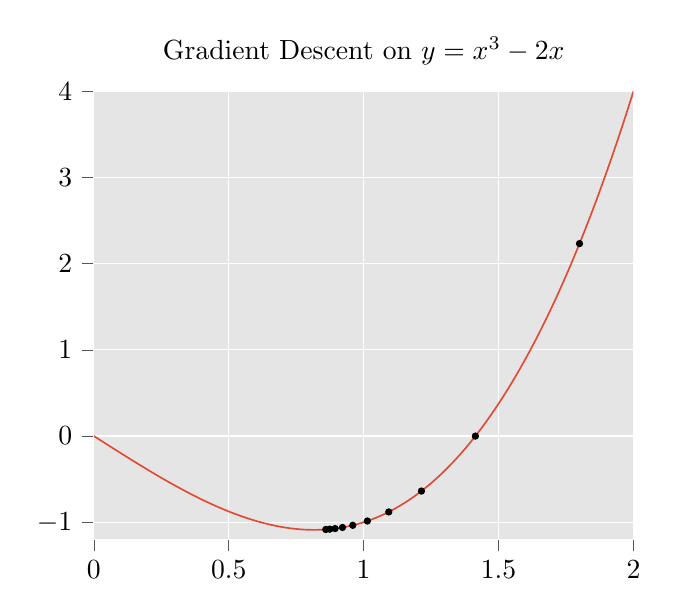
\begin{tikzpicture}

\definecolor{color0}{rgb}{0.886274509803922,0.290196078431373,0.2}

\begin{axis}[
axis background/.style={fill=white!89.8039215686275!black},
axis line style={white},
tick align=outside,
tick pos=left,
title={Gradient Descent on $y=x^3-2x$},
x grid style={white},
xmajorgrids,
xmin=0, xmax=2,
xtick style={color=white!33.3333333333333!black},
y grid style={white},
ymajorgrids,
ymin=-1.2, ymax=4,
ytick style={color=white!33.3333333333333!black}
]
\addplot [semithick, color0]
table {%
0 0
0.0202020201832056 -0.0403957962989807
0.0404040403664112 -0.0807421207427979
0.060606062412262 -0.120989516377449
0.0808080807328224 -0.161088496446609
0.101010099053383 -0.200989589095116
0.121212124824524 -0.240643352270126
0.141414135694504 -0.280000269412994
0.161616161465645 -0.319010943174362
0.181818187236786 -0.357625842094421
0.202020198106766 -0.395795524120331
0.222222223877907 -0.433470517396927
0.242424249649048 -0.470601350069046
0.262626260519028 -0.50713849067688
0.282828271389008 -0.543032586574554
0.30303031206131 -0.578234136104584
0.32323232293129 -0.612693607807159
0.34343433380127 -0.646361589431763
0.363636374473572 -0.67918860912323
0.383838385343552 -0.711125135421753
0.404040396213531 -0.742121756076813
0.424242436885834 -0.772128999233246
0.444444447755814 -0.801097393035889
0.464646458625793 -0.828977465629578
0.484848499298096 -0.855719745159149
0.505050480365753 -0.881274700164795
0.525252521038055 -0.905593037605286
0.545454561710358 -0.928625106811523
0.565656542778015 -0.950321435928345
0.585858583450317 -0.970632791519165
0.60606062412262 -0.989509463310242
0.626262605190277 -1.00690197944641
0.646464645862579 -1.0227609872818
0.666666686534882 -1.03703701496124
0.686868667602539 -1.04968059062958
0.707070708274841 -1.06064212322235
0.727272748947144 -1.06987226009369
0.747474730014801 -1.07732152938843
0.767676770687103 -1.08294034004211
0.787878811359406 -1.08667945861816
0.808080792427063 -1.08848929405212
0.828282833099365 -1.08832025527954
0.848484873771667 -1.08612298965454
0.868686854839325 -1.08184790611267
0.888888895511627 -1.07544589042664
0.909090936183929 -1.06686699390411
0.929292917251587 -1.05606210231781
0.949494957923889 -1.04298162460327
0.969696998596191 -1.02757596969604
0.989898979663849 -1.00979590415955
1.01010096073151 -0.989591956138611
1.03030300140381 -0.966914415359497
1.05050504207611 -0.941713929176331
1.07070708274841 -0.913940906524658
1.09090912342072 -0.883546233177185
1.11111116409302 -0.850480079650879
1.13131308555603 -0.814693212509155
1.15151512622833 -0.776136040687561
1.17171716690063 -0.734759092330933
1.19191920757294 -0.690512895584106
1.21212124824524 -0.643347978591919
1.23232328891754 -0.593214869499207
1.25252521038055 -0.540064573287964
1.27272725105286 -0.48384690284729
1.29292929172516 -0.424512386322021
1.31313133239746 -0.362012147903442
1.33333337306976 -0.296296119689941
1.35353529453278 -0.227315664291382
1.37373733520508 -0.155020475387573
1.39393937587738 -0.0793612003326416
1.41414141654968 -0.000288724899291992
1.43434345722198 0.0822467803955078
1.45454549789429 0.168294668197632
1.4747474193573 0.257903814315796
1.4949494600296 0.35112452507019
1.5151515007019 0.448006153106689
1.53535354137421 0.548598051071167
1.55555558204651 0.652949333190918
1.57575762271881 0.761110067367554
1.59595954418182 0.873128652572632
1.61616158485413 0.989055633544922
1.63636362552643 1.10894083976746
1.65656566619873 1.23283243179321
1.67676770687103 1.3607804775238
1.69696974754333 1.49283504486084
1.71717166900635 1.62904405593872
1.73737370967865 1.76945853233337
1.75757575035095 1.91412734985352
1.77777779102325 2.0631000995636
1.79797983169556 2.21642637252808
1.81818187236786 2.37415528297424
1.83838379383087 2.53633522987366
1.85858583450317 2.70301818847656
1.87878787517548 2.87425208091736
1.89898991584778 3.05008697509766
1.91919195652008 3.23057150840759
1.93939399719238 3.41575574874878
1.9595959186554 3.60568809509277
1.9797979593277 3.80042004585266
2 4
};
\addplot [semithick, black, mark=*, mark size=1, mark options={solid}, only marks]
table {%
1.79999995231628 2.23199939727783
1.41400003433228 -0.000854015350341797
1.21409058570862 -0.63859224319458
1.09298825263977 -0.880267262458801
1.01379477977753 -0.985631704330444
0.95962780714035 -1.03554821014404
0.921494960784912 -1.06049966812134
0.894122004508972 -1.07343447208405
0.874203860759735 -1.08031272888184
0.859569013118744 -1.08403778076172
};
\end{axis}

\end{tikzpicture}

        \caption{Demonstration of gradient descent convergence: 10 iterations with $\alpha =5\times 10^{-2}$ and $\theta_0=1.8$.}%
        \label{fig:gradient_demo}
\end{figure}

\subsubsection{Partial Derivative of Loss Function}%
\label{ssub:derivative_of_loss_function}
A partial derivative is the derivative of a multi-variable function \wrt{} a single variable, and is denoted by $\frac{\delta}{\delta x}$ instead of $\frac{d}{dx}$. Hence, our goal is to find the Jacobian matrix $\bm{J}$ of $L(S)$ \wrt{} $S$, defined as follows:
 \begin{align*}
     \bm{J}=\frac{\delta L(S)}{\delta S}= \begin{bmatrix}
                 \frac{\delta L(S)}{\delta S_{1,1}}&\cdots &\frac{\delta L(S)}{\delta S_{1,N^2}}\\
                 \vdots &\ddots &\vdots \\
                 \frac{\delta L(S)}{\delta S_{N^2,1}}&\cdots &\frac{\delta L(S)}{\delta S_{N^2,N^2}}\\
         \end{bmatrix}
\end{align*}

To do that, we need to find the general solution to the partial derivative: $ \frac{\delta L(S)}{\delta S_{i,j}}$. Recall that the loss function is defined as
\begin{align*}
    L(S)=\frac{1}{2}\sum_{a}^{N^2} \sum_{b}^{N^2} \sum_{c}^{N^2} \sum_{d}^{N^2} S_{a,b} S_{c,d} C(O)_{a,c}C(O)_{b,d}
\end{align*}
When evaluating $J_{i,j}$, only $S_{i,j}$ is treated as a variable, others are treated as constants. $S_{i,j}$ is only included within the loss when $(a,b)=(i,j)$ or $(c,d)=(i,j)$ or both. The derivatives for the respective cases are as follows:
\begin{align*}
        \bm{A}=\frac{\delta L(S)}{\delta S_{i,j}}&=\frac{\delta}{\delta S_{i,j}}\left(\frac{1}{2}\sum_{c}^{N^2} \sum_{d}^{N^2} S_{i,j} S_{c,d} C(O)_{i,c}C(O)_{j,d}\right)&\text{first case}\\
              &=\frac{1}{2}\sum_{c}^{N^2} \sum_{d}^{N^2} S_{c,d} C(O)_{i,c}C(O)_{j,d}&\\
        \bm{B}=\frac{\delta L(S)}{\delta S_{i,j}}&=\frac{\delta}{\delta S_{i,j}}\left(\frac{1}{2}\sum_{a}^{N^2} \sum_{b}^{N^2} S_{a,b} S_{i,j} C(O)_{a,i}C(O)_{b,j}\right)&\text{second case}\\
              &=\frac{1}{2}\sum_{a}^{N^2} \sum_{b}^{N^2} S_{a,b} C(O)_{a,i}C(O)_{b,j}&\\
        \bm{C}=\frac{\delta L(S)}{\delta S_{i,j}}&=\frac{\delta}{\delta S_{i,j}}\left(\frac{1}{2}S_{a,b} S_{a,b} C(O)_{a,b}C(O)_{a,b}\right)&\text{third case}\\
              &=\frac{1}{2}\sum_{a}^{N^2} \sum_{b}^{N^2} S_{a,b} C(O)_{a,a}C(O)_{b,b}&\\
              &=0&
\end{align*}
$\bm{C}$ is $0$ due because it includes the distance of a token against itself. The partial derivative of $L(S)$ \wrt{} $S_{i,j}$ is therefore equal to $\bm{A}+\bm{B}-\bm{C}=\bm{A}+\bm{B}$, because they encapsulate all of the cases where $S_{i,j}$ is a part of a term. A naive approach would be to update the entries as follows:
\begin{align*}
        S_{i,j}'=S_{i,j}-\alpha \left(\bm{A}+\bm{B}\right)
\end{align*}

\subsection{Generalization of Discrete Constraints}%
\label{sub:constraints}

\subsubsection{Doubly Stochastic Matrices}%
\label{ssub:doubly_stochastic_matrices}
First of all, regardless of whether discrete grids or superposition grids are involved, \emph{negative weights do not make sense}, as weights represent what portion of the token is located within a certain position.

Within $X$ or $O$, every position has a \emph{single} unique token, and every token has a \emph{single} unique position. To put it another way, no token does not have a position, and no position does not have a token. Note the superposition of a discrete grid in \ref{fig:superpositionShade}, the sums of all the rows and columns are equal to 1. In other words, the sum of all the weights within every position is 1, and the sum of all the weights of every token is 1. That is, a matrix $A$ with non-negative values and
\begin{align*}
    \sum_i A_{i,j}=\sum_j A_{i,j}=1
\end{align*}
is called a doubly stochastic matrix.\cite{weissteinDoubly} Therefore, the superposition $S$ must always be doubly stochastic.

\subsubsection{Sinkhorn-Knopp Algorithm}%
\label{ssub:sinkhorn_knopp_algorithm}
This section explains the algorithm used within \ref{ssub:zero_line_sum_modified_jacobian}.
A well-known algorithm to convert any non-negative matrix into a doubly stochastic matrix is called the Sinkhorn-Knopp algorithm (also named RAS).\cite{sinkhorn1967concerning} There is a proof\cite{borobia1998matrix} and several papers\cite{chakrabarty2018better,knight2008sinkhorn} analyzing its convergence. Nonetheless, the algorithm itself is simple: repetitively normalizing the rows and columns of a matrix.

Let $K$ be an $n\times n$ non-negative matrix.\footnote{every row and column should contain at least 1 positive value} A single iteration of RAS is defined as follows:

\begin{align*}
        K'=&\begin{bmatrix}
                (\Sigma_j^N K_{1,j})^{-1}\\
                &\ddots{}\\
                &&(\Sigma_j^N K_{N,j})^{-1}
        \end{bmatrix}K &&\text{normalizing rows}\\
            \text{RAS}(K)=K''=K'&\begin{bmatrix}
                (\Sigma_i^N K'_{i,1})^{-1}\\
                &\ddots{}\\
                &&(\Sigma_i^N K'_{i,N})^{-1}
        \end{bmatrix}&&\text{normalizing columns}
\end{align*}
The scaling matrices are diagonal (non-diagonal elements are $0$s). Here, ``normalizing'' is defined as forming a sum of 1. \autoref{fig:ras_demo} demonstrates the effectiveness of RAS. Graphed on the y-axis is the squared error, defined as:
\begin{align*}
        E(X)=\sum^N_i\left(\left(\sum^N_jX_{i,j}\right)-1\right)^2+\sum^N_j\left(\left(\sum^N_iX_{i,j}\right)-1\right)^2
\end{align*}
Although this does not prove the convergence of RAS, it demonstrates its effectiveness.

\begin{figure}[htpb]
        \centering
        % This file was created by tikzplotlib v0.9.1.
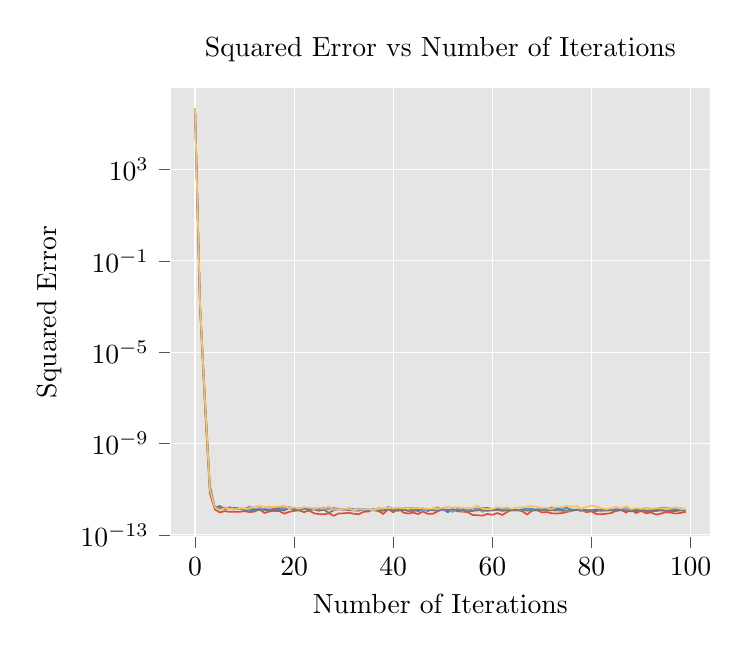
\begin{tikzpicture}

\definecolor{color0}{rgb}{0.886274509803922,0.290196078431373,0.2}
\definecolor{color1}{rgb}{0.203921568627451,0.541176470588235,0.741176470588235}
\definecolor{color2}{rgb}{0.596078431372549,0.556862745098039,0.835294117647059}
\definecolor{color3}{rgb}{0.984313725490196,0.756862745098039,0.368627450980392}

\begin{axis}[
axis background/.style={fill=white!89.8039215686275!black},
axis line style={white},
log basis y={10},
tick align=outside,
tick pos=left,
title={Squared Error vs Number of Iterations},
x grid style={white},
xlabel={Number of Iterations},
xmajorgrids,
xmin=-4.95, xmax=103.95,
xtick style={color=white!33.3333333333333!black},
y grid style={white},
ylabel={Squared Error},
ymajorgrids,
ymin=8.68476415176487e-14, ymax=3811887.27502007,
ymode=log,
ytick style={color=white!33.3333333333333!black}
]
\addplot [semithick, color0]
table {%
0 481023.09375
1 0.00103783328086138
2 4.61336888690767e-08
3 6.49791331852612e-12
4 1.31095134747738e-12
5 9.52127265918534e-13
6 1.09423581307055e-12
7 1.00541797110054e-12
8 1.02673425317334e-12
9 1.01252339845814e-12
10 1.07647224467655e-12
11 9.9120711638534e-13
12 1.03739239420975e-12
13 1.32516220219259e-12
14 9.05941988094128e-13
15 1.04805053524615e-12
16 1.11555209514336e-12
17 1.09778852674935e-12
18 8.41993141875719e-13
19 1.01607611213694e-12
20 1.10844666778576e-12
21 1.21502807814977e-12
22 9.80548975348938e-13
23 1.15818465928896e-12
24 8.77520278663724e-13
25 8.06466005087714e-13
26 7.85149723014911e-13
27 8.81072992342524e-13
28 6.78568312650896e-13
29 8.63309423948522e-13
30 8.73967564984923e-13
31 9.2370555648813e-13
32 8.38440428196918e-13
33 7.88702436693711e-13
34 1.01607611213694e-12
35 1.05160324892495e-12
36 1.30029320644098e-12
37 1.10489395410696e-12
38 8.20676859802916e-13
39 1.35358391162299e-12
40 9.62785406954936e-13
41 1.45661260830821e-12
42 9.52127265918534e-13
43 8.4909856923332e-13
44 9.41469124882133e-13
45 8.13571432445315e-13
46 1.04805053524615e-12
47 8.24229573481716e-13
48 8.31335000839317e-13
49 1.07291953099775e-12
50 1.33937305690779e-12
51 1.02673425317334e-12
52 1.31095134747738e-12
53 1.08357767203415e-12
54 1.03028696685215e-12
55 9.87654402706539e-13
56 7.42517158869305e-13
57 7.21200876796502e-13
58 6.89226453687297e-13
59 8.17124146124115e-13
60 7.49622586226906e-13
61 8.95283847057726e-13
62 7.38964445190504e-13
63 9.98312543742941e-13
64 1.26831878333178e-12
65 1.22213350550737e-12
66 1.08002495835535e-12
67 7.74491581978509e-13
68 1.13331566353736e-12
69 1.18660636871937e-12
70 9.55679979597335e-13
71 9.87654402706539e-13
72 8.73967564984923e-13
73 8.56203996590921e-13
74 8.91731133378926e-13
75 9.80548975348938e-13
76 1.16529008664656e-12
77 1.25766064229538e-12
78 1.17594822768297e-12
79 9.9120711638534e-13
80 1.05870867628255e-12
81 8.13571432445315e-13
82 7.92255150372512e-13
83 8.38440428196918e-13
84 8.88178419700125e-13
85 1.15107923193136e-12
86 1.21858079182857e-12
87 9.37916411203332e-13
88 1.29674049276218e-12
89 8.91731133378926e-13
90 1.11555209514336e-12
91 8.81072992342524e-13
92 9.48574552239734e-13
93 7.67386154620908e-13
94 8.4909856923332e-13
95 9.69890834312537e-13
96 9.41469124882133e-13
97 8.45545855554519e-13
98 9.09494701772928e-13
99 1.00186525742174e-12
};
\addplot [semithick, color1]
table {%
0 487870.4375
1 0.00108947034459561
2 5.42636904299343e-08
3 8.494538406012e-12
4 1.52766688188422e-12
5 1.48148160405981e-12
6 1.54187773659942e-12
7 1.4175327578414e-12
8 1.51345602716901e-12
9 1.48148160405981e-12
10 1.24700250125898e-12
11 1.23279164654377e-12
12 1.21858079182857e-12
13 1.4495071809506e-12
14 1.23989707390137e-12
15 1.28252963804698e-12
16 1.32871491587139e-12
17 1.18660636871937e-12
18 1.32160948851379e-12
19 1.4459544672718e-12
20 1.36779476633819e-12
21 1.4281908988778e-12
22 1.57740487338742e-12
23 1.25766064229538e-12
24 1.4281908988778e-12
25 1.34292577058659e-12
26 1.52056145452661e-12
27 1.4033219031262e-12
28 1.47082346302341e-12
29 1.31095134747738e-12
30 1.27542421068938e-12
31 1.4175327578414e-12
32 1.32160948851379e-12
33 1.19015908239817e-12
34 1.27897692436818e-12
35 1.20081722343457e-12
36 1.31805677483499e-12
37 1.14397380457376e-12
38 1.36424205265939e-12
39 1.26121335597418e-12
40 1.29674049276218e-12
41 1.13686837721616e-12
42 1.33937305690779e-12
43 1.11199938146456e-12
44 1.37845290737459e-12
45 1.06936681731895e-12
46 1.37134748001699e-12
47 1.08357767203415e-12
48 1.4317436125566e-12
49 1.17239551400417e-12
50 1.33937305690779e-12
51 9.73443547991337e-13
52 1.29318777908338e-12
53 1.07291953099775e-12
54 1.35358391162299e-12
55 1.11555209514336e-12
56 1.4459544672718e-12
57 1.33582034322899e-12
58 1.46016532198701e-12
59 1.50990331349021e-12
60 1.35713662530179e-12
61 1.35713662530179e-12
62 1.424638185199e-12
63 1.3997691894474e-12
64 1.31805677483499e-12
65 1.19371179607697e-12
66 1.28252963804698e-12
67 1.406874616805e-12
68 1.35358391162299e-12
69 1.25766064229538e-12
70 1.34647848426539e-12
71 1.35003119794419e-12
72 1.56319401867222e-12
73 1.3962164757686e-12
74 1.54543045027822e-12
75 1.49213974509621e-12
76 1.25055521493778e-12
77 1.27187149701058e-12
78 1.26831878333178e-12
79 1.21502807814977e-12
80 1.15107923193136e-12
81 1.06936681731895e-12
82 1.29318777908338e-12
83 1.32160948851379e-12
84 1.16529008664656e-12
85 1.12976294985856e-12
86 1.19015908239817e-12
87 1.14042109089496e-12
88 1.05870867628255e-12
89 1.09778852674935e-12
90 1.16173737296776e-12
91 1.10844666778576e-12
92 1.06936681731895e-12
93 1.10134124042816e-12
94 1.16173737296776e-12
95 1.10844666778576e-12
96 1.06936681731895e-12
97 1.10134124042816e-12
98 1.16173737296776e-12
99 1.10844666778576e-12
};
\addplot [semithick, color2]
table {%
0 483571.625
1 0.00135559169575572
2 9.83107923957505e-08
3 1.40119027491892e-11
4 1.68753899743024e-12
5 1.68753899743024e-12
6 1.27897692436818e-12
7 1.66267000167863e-12
8 1.34647848426539e-12
9 1.389111048411e-12
10 1.3962164757686e-12
11 1.74082970261225e-12
12 1.33582034322899e-12
13 1.47082346302341e-12
14 1.33582034322899e-12
15 1.72306613421824e-12
16 1.45661260830821e-12
17 1.55253587763582e-12
18 1.47082346302341e-12
19 1.65201186064223e-12
20 1.29674049276218e-12
21 1.31450406115619e-12
22 1.30384592011978e-12
23 1.49569245877501e-12
24 1.30739863379858e-12
25 1.33937305690779e-12
26 1.22568621918617e-12
27 1.36424205265939e-12
28 1.3962164757686e-12
29 1.4175327578414e-12
30 1.23279164654377e-12
31 1.424638185199e-12
32 1.15463194561016e-12
33 1.4139800441626e-12
34 1.23989707390137e-12
35 1.29674049276218e-12
36 1.16529008664656e-12
37 1.47082346302341e-12
38 1.35358391162299e-12
39 1.66977542903624e-12
40 1.389111048411e-12
41 1.53121959556302e-12
42 1.4459544672718e-12
43 1.51345602716901e-12
44 1.47437617670221e-12
45 1.48148160405981e-12
46 1.16173737296776e-12
47 1.30029320644098e-12
48 1.29674049276218e-12
49 1.60937929649663e-12
50 1.16529008664656e-12
51 1.29674049276218e-12
52 1.00541797110054e-12
53 1.4281908988778e-12
54 1.03739239420975e-12
55 1.29318777908338e-12
56 1.08713038571295e-12
57 1.4530598946294e-12
58 1.01252339845814e-12
59 1.27542421068938e-12
60 1.15107923193136e-12
61 1.21147536447097e-12
62 1.08357767203415e-12
63 1.18305365504057e-12
64 1.14397380457376e-12
65 1.14752651825256e-12
66 1.25055521493778e-12
67 1.30029320644098e-12
68 1.17950094136177e-12
69 1.33582034322899e-12
70 1.18305365504057e-12
71 1.21147536447097e-12
72 1.17594822768297e-12
73 1.16173737296776e-12
74 1.11199938146456e-12
75 1.04094510788855e-12
76 1.08002495835535e-12
77 1.23989707390137e-12
78 1.06226138996135e-12
79 1.14752651825256e-12
80 1.14042109089496e-12
81 1.31805677483499e-12
82 1.04805053524615e-12
83 1.26831878333178e-12
84 1.19726450975577e-12
85 1.36424205265939e-12
86 1.27542421068938e-12
87 1.442401753593e-12
88 1.19726450975577e-12
89 1.30384592011978e-12
90 1.27187149701058e-12
91 1.47082346302341e-12
92 1.3997691894474e-12
93 1.38200562105339e-12
94 1.53121959556302e-12
95 1.53477230924182e-12
96 1.3855583347322e-12
97 1.4495071809506e-12
98 1.4530598946294e-12
99 1.22213350550737e-12
};
\addplot [semithick, white!46.6666666666667!black]
table {%
0 477859.46875
1 0.00130087230354548
2 9.17595883720423e-08
3 1.25766064229538e-11
4 1.50635059981141e-12
5 1.83320025826106e-12
6 1.37845290737459e-12
7 1.53477230924182e-12
8 1.29318777908338e-12
9 1.48148160405981e-12
10 1.12265752250096e-12
11 1.406874616805e-12
12 1.21858079182857e-12
13 1.22213350550737e-12
14 1.24344978758018e-12
15 1.12621023617976e-12
16 1.4281908988778e-12
17 1.37845290737459e-12
18 1.14397380457376e-12
19 1.51700874084781e-12
20 1.23634436022257e-12
21 1.14397380457376e-12
22 1.48503431773861e-12
23 1.18660636871937e-12
24 1.30384592011978e-12
25 1.12621023617976e-12
26 1.26476606965298e-12
27 9.2370555648813e-13
28 1.17594822768297e-12
29 1.31805677483499e-12
30 1.34292577058659e-12
31 1.19726450975577e-12
32 1.17239551400417e-12
33 1.13686837721616e-12
34 1.32871491587139e-12
35 1.27542421068938e-12
36 1.18660636871937e-12
37 1.11910480882216e-12
38 1.14042109089496e-12
39 1.32871491587139e-12
40 1.18660636871937e-12
41 1.15818465928896e-12
42 1.22568621918617e-12
43 1.14397380457376e-12
44 1.07647224467655e-12
45 1.25766064229538e-12
46 1.4210854715202e-12
47 1.35358391162299e-12
48 1.17239551400417e-12
49 1.13686837721616e-12
50 1.32516220219259e-12
51 1.20792265079217e-12
52 1.31095134747738e-12
53 1.17594822768297e-12
54 1.21502807814977e-12
55 1.01607611213694e-12
56 1.11910480882216e-12
57 1.17594822768297e-12
58 1.23634436022257e-12
59 1.11199938146456e-12
60 1.20081722343457e-12
61 1.22568621918617e-12
62 1.25410792861658e-12
63 1.14042109089496e-12
64 1.20081722343457e-12
65 1.22568621918617e-12
66 1.25410792861658e-12
67 1.14042109089496e-12
68 1.20081722343457e-12
69 1.22568621918617e-12
70 1.25410792861658e-12
71 1.14042109089496e-12
72 1.20081722343457e-12
73 1.22568621918617e-12
74 1.25410792861658e-12
75 1.14042109089496e-12
76 1.20081722343457e-12
77 1.22568621918617e-12
78 1.25410792861658e-12
79 1.14042109089496e-12
80 1.20081722343457e-12
81 1.22568621918617e-12
82 1.25410792861658e-12
83 1.14042109089496e-12
84 1.20081722343457e-12
85 1.22568621918617e-12
86 1.25410792861658e-12
87 1.14042109089496e-12
88 1.20081722343457e-12
89 1.22568621918617e-12
90 1.25410792861658e-12
91 1.14042109089496e-12
92 1.20081722343457e-12
93 1.22568621918617e-12
94 1.25410792861658e-12
95 1.14042109089496e-12
96 1.20081722343457e-12
97 1.22568621918617e-12
98 1.25410792861658e-12
99 1.14042109089496e-12
};
\addplot [semithick, color3]
table {%
0 477847.34375
1 0.00137645937502384
2 7.78547857294143e-08
3 9.65627577897976e-12
4 1.59161572810262e-12
5 1.18660636871937e-12
6 1.47437617670221e-12
7 1.4210854715202e-12
8 1.28963506540458e-12
9 1.51345602716901e-12
10 1.37490019369579e-12
11 1.4104273304838e-12
12 1.70174985214544e-12
13 1.88293824976427e-12
14 1.64490643328463e-12
15 1.67332814271504e-12
16 1.63780100592703e-12
17 1.75148784364865e-12
18 1.86517468137026e-12
19 1.4388490399142e-12
20 1.61648472385423e-12
21 1.4104273304838e-12
22 1.58451030074502e-12
23 1.59161572810262e-12
24 1.35003119794419e-12
25 1.57029944602982e-12
26 1.3997691894474e-12
27 1.77990955307905e-12
28 1.25766064229538e-12
29 1.31095134747738e-12
30 1.37134748001699e-12
31 1.3926637620898e-12
32 1.20436993711337e-12
33 1.30384592011978e-12
34 1.29674049276218e-12
35 1.33582034322899e-12
36 1.20081722343457e-12
37 1.3997691894474e-12
38 1.45661260830821e-12
39 1.51345602716901e-12
40 1.406874616805e-12
41 1.55253587763582e-12
42 1.4352963262354e-12
43 1.4495071809506e-12
44 1.4317436125566e-12
45 1.47082346302341e-12
46 1.4459544672718e-12
47 1.36424205265939e-12
48 1.4175327578414e-12
49 1.36779476633819e-12
50 1.52411416820541e-12
51 1.66977542903624e-12
52 1.57740487338742e-12
53 1.64490643328463e-12
54 1.52411416820541e-12
55 1.56319401867222e-12
56 1.45661260830821e-12
57 1.91491267287347e-12
58 1.3855583347322e-12
59 1.35358391162299e-12
60 1.36068933898059e-12
61 1.59872115546023e-12
62 1.46016532198701e-12
63 1.55964130499342e-12
64 1.37490019369579e-12
65 1.60227386913903e-12
66 1.55608859131462e-12
67 1.75504055732745e-12
68 1.79767312147305e-12
69 1.69109171110904e-12
70 1.48858703141741e-12
71 1.54187773659942e-12
72 1.37134748001699e-12
73 1.63069557856943e-12
74 1.60582658281783e-12
75 1.84741111297626e-12
76 1.65911728799983e-12
77 1.78701498043665e-12
78 1.36068933898059e-12
79 1.70530256582424e-12
80 1.85451654033386e-12
81 1.79412040779425e-12
82 1.46016532198701e-12
83 1.34647848426539e-12
84 1.48858703141741e-12
85 1.65556457432103e-12
86 1.4459544672718e-12
87 1.76925141204265e-12
88 1.31450406115619e-12
89 1.49569245877501e-12
90 1.36779476633819e-12
91 1.49924517245381e-12
92 1.36068933898059e-12
93 1.46016532198701e-12
94 1.424638185199e-12
95 1.38200562105339e-12
96 1.4530598946294e-12
97 1.59872115546023e-12
98 1.35358391162299e-12
99 1.31805677483499e-12
};
\end{axis}

\end{tikzpicture}

        \caption{Demonstration of RAS convergence: 5 samples with $N=100$, randomly generated from a uniform distribution $[0,\frac{2}{N})$ (mean $\frac{1}{N}$ ). Error is equal to the sum of squared errors of the sums of the rows and columns from 1. Note the logarithmic scale.}%
        \label{fig:ras_demo}
\end{figure}

Another example of the RAS algorithm:
\begin{align*}
    K=&\begin{bmatrix}
        0&2&4\\
        1&3&5\\
        2&4&6
    \end{bmatrix}\\
    K'=
    \begin{bmatrix}
        \frac{1}{6}&0&0\\
        0&\frac{1}{9} &0\\
        0&0&\frac{1}{12}
    \end{bmatrix}
     &\begin{bmatrix}
        0&2&4\\
        1&3&5\\
        2&4&6
    \end{bmatrix}=
    \begin{bmatrix}
        0&\frac{1}{3}&\frac{2}{3}\\[4pt]
        \frac{1}{9}&\frac{1}{3}&\frac{5}{9}\\[4pt]
        \frac{1}{6}&\frac{1}{3}&\frac{1}{2}
    \end{bmatrix}\\
    \text{RAS}(K)=K''=
     &\begin{bmatrix}
         0&\frac{1}{3}&\frac{2}{3}\\[4pt]
         \frac{1}{9}&\frac{1}{3}&\frac{5}{9}\\[4pt]
        \frac{1}{6}&\frac{1}{3}&\frac{1}{2}
    \end{bmatrix}
    \begin{bmatrix}
         \frac{18}{5}&0&0\\
         0&1&0\\
         0&0&\frac{18}{31}
    \end{bmatrix}=
    \begin{bmatrix}
        0&\frac{1}{3}&\frac{12}{31}\\[4pt]
        \frac{2}{5}&\frac{1}{3}&\frac{10}{31}\\[4pt]
        \frac{3}{5}&\frac{1}{3}&\frac{9}{31}
    \end{bmatrix}
\end{align*}

\subsubsection{Zero Line-Sum Modified Jacobian}%
\label{ssub:zero_line_sum_modified_jacobian}
To maintain the doubly stochastic nature of the superposition grid within gradient descent update (in \ref{ssub:derivative_of_loss_function}), the Jacobian matrix must be modified into a zero line-sum (ZLS) matrix.\cite{zeroLineSum} A ZLS matrix has all rows and columns summing to 1, that is, a matrix $A$ is ZLS iff.
\begin{align*}
    \sum_i A_{i,j}=\sum_j A_{i,j}=0
\end{align*}

As stated within \cite{zeroLineSum}, a ZLS can be obtained by taking the difference of 2 doubly stochastic matrices.
\begin{proof}
    Let $A$ and $B$ be doubly stochastic matrices.
    \begin{align*}
        \sum_i \left(A_{i,j}-B_{i,j}\right)= \sum_i A_{i,j}-\sum_i B_{i,j}=1-1=0\\
        \sum_j \left(A_{i,j}-B_{i,j}\right)= \sum_j A_{i,j}-\sum_j B_{i,j}=1-1=0
    \end{align*}
    Therefore, $A-B$ is doubly stochastic.
\end{proof}

Hence, a Jacobian can be converted into a doubly stochastic matrix through the RAS algorithm,\footnote{the Jacobian of the loss function is non-negative because $S$ and $C(O)$ are non-negative, so RAS is applicable} and by subtracting it by another doubly stochastic matrix, a ZLS-Jacobian can be obtained. This second doubly stochastic matrix can be obtained by scaling a ones-matrix (matrix filled with ones). Let this second doubly stochastic matrix be $D$ with dimension $N\times N$. $D$ is defined as follows:
\begin{align*}
    D_{i,j}&=\frac{1}{N}\\
    \sum_i D_{i,j}&=\sum_j D_{i,j}=N\times \frac{1}{N}=1 &\text{$D$ is doubly stochastic}
\end{align*}
Because $D$ is uniform (all elements have identical values), the magnitudes of the elements doubly stochastic Jacobian elements \wrt{} other elements are preserved, that is $\text{RAS}(J)_{a,b}>\text{RAS}(J)_{c,d} \iff \text{RAS}(J)_{a,b}-D_{a,b}>\text{RAS}(J)_{c,d}-D_{c,d}$

Let $J'=\text{RAS}(J)-D$.

\subsubsection{Non-negative Matrices}%
\label{ssub:non_negative_matrices}
Assuming $S$ is doubly stochastic, and with ZLS-$J'$, the result of the gradient descent update $S'=S-\alpha J'$, has rows and columns summing to 1. \emph{But $S'$ is not necessarily doubly stochastic, because $S'$ might not be non-negative}. Given that $S'$ has dimension $N^2\times N^2$ the following procedure corrects negative entries while still maintaining the rows and columns summing to 1, effectively ensuring that $S'$ is doubly stochastic:

\begin{align*}
 S''_{i,j}=
\begin{cases}
    (S'_{i,j}+\min{S})\times \frac{1}{1+N^2 \min{S}} & \exists a,b\quad S'_{a,b}<0\\
    S'_{i,j} & \nexists a,b\quad S'_{a,b}<0
\end{cases}
\end{align*}
$\min{S'}$ refers to the smallest value within $S'$. $S'_{i,j}+\min{S}$ effectively creates a non-negative matrix.\footnote{$\exists a,b\quad S'_{a,b}<0$ means ``exists $a,b$ such that $S'_{a,b}$ is negative''}

\begin{proof}
    Let $S'$ be a matrix with rows and columns summing to 1.
    \begin{align*}
        \sum_i^{N^2} S''_{i,j}&=\sum_i^{N^2} (S'_{i,j}+\min{S})\times \frac{1}{1+N^2 \min{S}}=\frac{1}{1+N^2 \min{S}} \sum_i^{N^2} (S'_{i,j}+\min{S})\\
                             &=\frac{1}{1+N^2 \min{S}} (\sum_i^{N^2} (S'_{i,j})+N^2\min{S})=\frac{1}{1+N^2 \min{S}} (1+N^2\min{S})\\
                       &=1
    \end{align*} Replace $\sum_i^{N^2}$ with $\sum_j^{N^2}$ and repeat. Therefore, $S''$ is doubly stochastic.
\end{proof}

With this, $S$ can be optimized by gradient descent.

\subsection{Generalization to Discrete Solutions}%
\label{sub:generalization_to_discrete_solutions}
Note that only the continuous representation $S$ has been optimized, and not the discrete solution $X$, which has been the goal of the essay. Expanding on the idea of quantum superposition within physics, by observing (or revealing) the position of an electron, the probability density function of the electron position collapses, being reduced to a single point. And because it relates with probabilities, the results are random, they are \emph{probabilistic}. Within this essay, the probability density function has been represented by the weights of fragments within various positions. But instead of sampling from a distribution, by revealing a token, it will be placed in the position of the fragment with the highest weight, ie. the most likely position.

Taking this analogy even further, the tokens are \emph{entangled}. In physics, if two electrons are entangled, when the \emph{spin}\footnote{a quantum property beyond the scope of this essay} of an electron is revealed, the other is also instantaneously revealed. If one is found to be spin up, the other electron has spin down, vice versa. The system within this essay involves $N$  ``electrons'' (tokens), and when the position of this is revealed, the fragments from other tokens within the same position are removed, because no two tokens should inhabit the same position.

Also, the fragments of revealed tokens (columns of $S$) and fragments within revealed positions (rows of $S$) should be optimized. Since revealed tokens and positions are \emph{fixed}.

The procedure for revealing a token is defined as follows Let $R=\emptyset$ be a set of indices (rows and columns) of revealed fragments.
\begin{align*}
    R\leftarrow R\cup \argmax_{(m,n)\notin R}S_{m,n}\\
    S_{i,j}=
    \begin{cases}
        S_{ij}
    \end{cases}
\end{align*}
$\argmax_{(m,n)\notin R}S_{m,n}$ returns the indices of the fragment with the highest weight, $a\leftarrow b$ indicates a reassignment: the new value of $a$ is $b$.

To only perform optimization on non-revealed token fragments and positions, the revealed rows and columns can be removed from $J$, the appropriate procedures can be performed to obtain $J'$, and the $J'$ can be expanded to its original dimensions $N^2\times N^2$, by filling the revealed rows and columns with $0$s, effectively preventing optimization of revealed rows and columns.

Note that the previous procedure only works when $\argmax$ is defined, \emph{when there are tokens to reveal}, when  $|R|<N$, where $|R|$ denotes the number of indices within $R$.

\subsection{Optimization Procedure}%
\label{sub:optimization_procedure}
\subsubsection{Superposition Initialization}%
\label{ssub:superposition_initialization}
Recall that for the optimization of $S$, $S$ must be doubly stochastic. When no tokens have been revealed, $S=D$ (from \ref{ssub:zero_line_sum_modified_jacobian}). To work with an arbitrary amount of revealed tokens, $S$ with dimensions $N^2 \times N^2$ is defined as follows:
\begin{align*}
S_{i,j}=
\begin{cases}
    \frac{1}{N-|R|}& \nexists a\enspace (a,j)\in R \land \nexists b\enspace (i,b)\in R\enspace \text{if neither $i$ or $j$ have been revealed}\\
    0& \exists a\enspace (a,j)\in R \oplus \exists b\enspace (i,b)\in R\enspace \text{if only one of $i$ or $j$ has been revealed}\\
    1& \exists a\enspace (a,j)\in R \land \exists b\enspace (i,b)\in R\enspace \text{if $i,j$ is a revealed token}
\end{cases}
\end{align*}

\begin{proof}
\emph{upcoming proof of double stochasticity}
\end{proof}

The following is the optimization procedure
\begin{enumerate}
    \item Initialize $S$
    \begin{enumerate}
    \item For every $N$:
        \begin{enumerate}
            \item For $n_{optim}$ steps:
    \begin{enumerate}
        \item Calculate $J$, ensure ZLS $J'$
        \item Perform gradient descent update
        \item Ensure doubly stochastic $S''$
    \end{enumerate}
    \item Reveal token
        \end{enumerate}
    \end{enumerate}
\end{enumerate}
